\documentclass[12pt]{article}   	% use "amsart" instead of "article" for AMSLaTeX format
\usepackage[letterpaper,bindingoffset=0.2in,%
            left=1.2in, right=1.2in, top=1.2in, bottom=1.2in,%
            footskip=.25in]{geometry}
%\geometry{landscape}                		% Activate for rotated page geometry
%\usepackage[parfill]{parskip}    		% Activate to begin paragraphs with an empty line rather than an indent
\usepackage{graphicx}				% Use pdf, png, jpg, or eps§ with pdflatex; use eps in DVI mode
								% TeX will automatically convert eps --> pdf in pdflatex

										
\usepackage{amssymb,amsmath,amsthm,enumitem}
\usepackage{setspace}
\usepackage{booktabs}
\usepackage{float}
\usepackage{endfloat}
\usepackage{natbib}
\usepackage{varioref}
\usepackage{geometry}
\usepackage{pdflscape}
\usepackage{rotating}
\usepackage{caption}
\usepackage{bbm}

\usepackage{makecell}
\renewcommand\theadfont{}


% \bibpunct{(}{)}{;}{a}{}{,}

\usepackage{etoolbox}
\newcommand{\zerodisplayskips}{%
  \setlength{\abovedisplayskip}{4pt}%
  \setlength{\belowdisplayskip}{4pt}%
  \setlength{\abovedisplayshortskip}{4pt}%
  \setlength{\belowdisplayshortskip}{4pt}}
\appto{\normalsize}{\zerodisplayskips}
\appto{\small}{\zerodisplayskips} 
\appto{\footnotesize}{\zerodisplayskips}

%SetFonts

\numberwithin{equation}{section}

\title{Mitigating Publication Bias Using Bayesian Stacking}
\author{Thomas A. Gibson}
%\date{}							% Activate to display a given date or no date

\begin{document}
\maketitle

\doublespacing
\nomarkersintext

\section{Introduction} \label{sec:intro}

Results from a meta-analysis may be skewed and unreliable in the presence of publication bias, where the publication or non-publication of a study depends on the statistical significance or magnitude of its results \citep{rothstein2006}. Statistical methods for publication bias have been designed for sensitivity analysis, testing for the presence/magnitude of publication bias, and calculating bias-corrected parameter estimates. Most methods are either based on the funnel plot or selection models.

Methods based on the funnel plot \citep{light1984funnel} -- a scatterplot of effect sizes against their standard errors -- inspect the plot's asymmetry to test or correct for bias. Say we have $S$ studies indexed by $i = 1,\dots,S$ and that ${y_i}$ and ${v_i} = {s_i^2}$ are their estimated effect sizes and sampling variances. A popular non-parametric test for publication bias \citep{begg1994test} measures the rank correlation between standardized observed effect sizes $y_i^*$ and the effect sizes' variances $v_i$, where 
\begin{align}
y_i^* &= (y_i - \overline{y}) / (v_i^*)^{1/2} \nonumber \\
\overline{y} &= \Big( \sum_j (v_i^{-1})/ y_i \Big) / \Big( \sum_j v_i^{-1} \Big) \nonumber \\
v_i^* &= v_i - \Big( \sum_j v_i^{-1} \Big)^{-1}. \nonumber
\end{align}
\citet{begg1994test} measure the correlation between pairs $(y_i^*, v_i)$ with Kendall's tau, where a symmetric funnel plot would have correlation near zero. Egger's test \citep{egger1997test} fits a linear regression of observed standard normal deviates $\text{SND}_i = y_i / s_i$ against the inverse standard errors $1 / s_i$, i.e. $\text{SND}_i = \alpha + \beta \times (1 / s_i)$  with the null hypothesis $H_0: \alpha = 0$. Other regression methods \citep{macaskill2001test, rucker2008arcsine, thompson1999test, peters2006test} are similar to Egger's test and use regression weights or transformations to improve upon Egger's test in the presence of heterogeneity or for dichotomous outcomes \citep{jin2015methods}. \citet{lin2018test} develops a measure for the severity of publication bias based on the skewness of standardized deviates. The trim-and-fill method \citep{duval2000biom} calculates an adjusted mean effect estimate in a series of steps, by 1) estimating the number of missing studies $k_0$, 2) ``trimming" the smaller studies that are causing funnel plot asymmetry, 3) estimating the true mean effect with the remaining studies, and 4) replacing trimmed studies and their missing counterparts and re-estimating the mean effect and its variance. However, \citet{duval2000biom} recommend using trim-and-fill as a sensitivity analysis based on the \textit{potential} number of missing studies, with general guidelines for sensitivity analysis given in \citet{shi2019trim}. The trim-and-fill method is the only funnel plot-based method that offers an adjusted mean estimate, and it is not recommended if there is heterogeneity in study effects \citep{jin2015methods}.

A second class of methods is based on \textit{selection models}, first described in \citet{hedges1984selection}. Let $Y$ be a random variable representing effect sizes for all studies in a population and let $\Theta$ be the parameters determining the sampling density $f(y;\Theta)$. Selection models assume a biased sampling scheme where the probability of a study being observed (published) is represented by a weight function $w(y; \lambda)$, where $\lambda$, a scalar or vector parameter, determines how certain studies may be more or less likely to be published. The weighted density for observed effect $y_i$ is then
\begin{equation}
f^*(y_i ;  \Theta, \lambda) = \frac{f(y_i;\Theta) w(y_i; \lambda)}{\int f(y ; \Theta) w(y; \lambda) dy}
\end{equation}
and the likelihood function for all observed studies is 
\begin{equation}
L(\Theta, \lambda) = \prod_{i = 1}^S f^*(y_i; \Theta, \lambda).
\end{equation}
Some models explicitly model the probability of publication for individual studies as a function of their p-values \citep{iyengar1988selection, hedges1992selection, givens1997, vevea1995pubbias} or as a function of both the effect size and standard error \citep{copas1999what, copas2000funnel, copas2001sensitivity}. \citet{hedges1992selection} introduced stepped weight functions by dividing the unit interval [0, 1] into $K$ segments with $K-1$ cut points, where studies that have $p$-values in different segments have different probabilities of publication. We refer to stepped selection functions by the number of cut points, i.e. a 1-step selection function might have a single cut point at $p=0.05$, or a 2-step function might have cuts at $p=0.05, 0.10$. Earlier selection models were recommended for bias-corrected effect size estimates, and were later recommended only for sensitivity analyses because of identifiability issues in smaller meta-analyses \citep{vevea2005sensitivity, jin2015methods}. Sensitivity analyses use a grid representing varying levels of publication bias and estimate the mean effect under each assumed scenario. If results do not change much under an assumption of severe publication bias they are robust, and if results do change under an assumption of mild publication bias they are sensitive. Bayesian implementations of the Copas selection model \citep{mavridis2013copas, bai2020} have again allowed for estimation of mean effect sizes.

Recent approaches to mitigating publication bias have used Bayesian model averaged meta-analysis (BMA-MA) to consider a set of potential selection functions. \citet{guan2016} considers four different selection functions based on $p$-values, including a no-bias model, an extreme-bias model where studies with p-values $p > \alpha$ are never published, a 1-step function where studies with $p > \alpha$ are published with some probability $\pi < 1$, and a model where the probability of publication decreases exponentially with $p$. \citet{guan2016} only implement the models in a fixed-effects framework. \citet{maier2020robma} evaluates a set of 12 models, using a $2 \times 2 \times 2$ factorial design with fixed/random effects, a true null/alternative hypothesis, and the presence/absence of publication bias. \citet{maier2020robma} fit two-step and three-step selection functions based on p-values when publication bias is assumed, where the probability of publication changes at $p=0.05$ (one-step) or at both $p = 0.05$ and $p = 0.10$ (two-step).  

Bayesian model averaging (BMA) effectively assumes that one of the considered models is the ``true" model, which is called the $\mathcal{M}$-closed setting \citep{bernardo2009}. BMA does not perform as well under the $\mathcal{M}$-complete or $\mathcal{M}$-open settings, where the true data generating mechanism is too complex to implement or to put into a probabilistic framework \citep{bernardo2009, le2017stacking}. Multiple issues arise for BMA in these settings, including (a) the need to specify prior model probabilities, which makes little sense when we know the true model is not in our list, and (b) the model weights from BMA will converge to 1 for the model ``closest" to the true model in terms of Kullback-Leibler divergence, and 0 for all others \citep{clyde2013bma}. Bayesian stacking of predictive distributions \citep{yao2018stacking, yao2021hierarchical} is a method that outperforms Bayesian model averaging in the $\mathcal{M}$-complete and $\mathcal{M}$-open settings and avoids issues (a) and (b) above. If we have $K$ candidate models $M_1, \dots, M_K$, \citet{yao2018stacking} solve for model weights $w = (w_1, \dots, w_K)$ under the constraint $w \in \mathcal{S}_1^K$ where $\mathcal{S}_1^K = \{w \in [0,1]^K : \sum_{k=1}^K w_k = 1\}$. They do this by solving
\begin{equation}
(\hat{w}_1, \dots, \hat{w}_K) =  \underset{w \in \mathcal{S}_1^K}{\mbox{max}} \: \frac{1}{S} \sum_{i = 1}^n \log \sum_{k = 1}^K w_k p(y_i \vert y_{-i}, M_k)
\end{equation}
where $p(y_i \vert y_{-i}, M_k)$ is the leave-one-out (LOO) posterior predictive density with the $i$th data point left out evaluated at $y_i$. It would be computationally costly to refit each model $M_k$ $S$ times, so LOO densities $p(y_i \vert y_{-i}, M_k)$ are approximated using Pareto-smoothed importance sampling \citep{vehtari2017psis}. We go through Bayesian stacking more thoroughly in Section \ref{sec:stacking}.

Given that the true data generating mechanism for publication bias is likely much too complex to be specified in a simple selection model, we propose using Bayesian stacking to mitigate publication bias by fitting multiple Bayesian selection models and stacking over them. Assumed patterns of publication bias that poorly predict the observed data with LOO cross validation will be given little weight. We propose stacking over multiple types of models, including step functions \citep{vevea1995pubbias} and Bayesian Copas selection models \citet{mavridis2013copas, bai2020}. Section \ref{sec:methods} describes relevant selection models for publication bias, Bayesian stacking, and how to implement Bayesian stacking of selection models. We then describe and summarize a simulation study in Section \ref{sec:simulation}. The purpose of the simulation is to compare a stacked estimate of the mean effect size to estimates from individual selection models when the true data generator is not one of the fitted selection models. We apply the stacked model to a real dataset on the effectiveness of antidepressants in Section \ref{sec:numex}

\section{Methods} \label{sec:methods}

We are doing a meta-analysis and have $S$ studies indexed by $i = 1, \dots, S$, and each study provides an estimated effect $y_i$ and an associated standard error $s_i$. Assuming estimates $y_i$ are normally distributed, we calculate study $i$'s 2-sided $p$-value as $p_i = 2 \times \big(1 - \Phi(\vert y_i \vert / s_i)\big)$ where $\Phi(\cdot)$ is the standard normal cumulative distribution function. The data model for each selection method is
\begin{align}
y_i & = \theta_i + s_i \epsilon_i \label{eq:y} \\
\theta_i \vert \theta, \tau ^ 2 & \sim \mbox{N}(\theta, \tau ^ 2) \label{eq:thetai}
\end{align}
where $\theta_i$ represent random study effects normally distributed around global mean $\theta$ with variance $\tau^2$, and $\epsilon_i \sim \text{N}(0, 1)$. For stepped weight functions we combine $s_i^2$ and $\tau^2$ into a single residual so that
\begin{align}
y_i \vert \theta, \tau^2 &\sim \text{N}(\theta, s_i^2 + \tau^2).
\end{align}

\subsection{Selection models based on p-values} \label{sec:pvalue}

We define a stepped weight function $w(\cdot)$ similar to \citet{vevea1995pubbias} and \citet{vevea2005sensitivity}, where $w(p)$ represents the probability that a study with $p$-value $p$ is observed. Dividing the unit interval into $K$ sub-intervals with descending endpoints $a_k$ in which the weight function $w(p)$ is constant, we have that
\begin{equation} % weight function
w(p_i) =
	\begin{cases}
		\omega_1 & \text{if $a_1 < p_i < 1$} \\
		\omega_j & \text{if $a_{j} < p_i < a_{j-1}$} \\
		\omega_K & \text{if $0 < p_i < a_{K-1}$}
	\end{cases} \label{eq:weight_fcn}
\end{equation}
where $a_0 = 1$ and $a_K = 0$. Say $\boldsymbol{\omega} = (\omega_1, \dots, \omega_K)$. We then have that the likelihood contribution for each observation $y_i$ given $\theta$, $\tau^2$ and weight function $w(\cdot)$ is 
\begin{equation} % weighted normal pdf
f(y_i \vert \theta, \tau^2, \boldsymbol{\omega}) = \frac{\phi(y_i ; \theta, \tau^2 + s_i^2) \times w(p_i)}{\int \phi(x ; \theta, \tau^2 + s_i^2) \times w(p(x, s_i)) dx}, \label{eq:weightednormal}
\end{equation}
where $\phi(x; a, b)$ represents a normal probability density function with mean $a$ and variance $b$, and $p(x, s_i) = 1 - \Phi(x / s_i)$ for one-sided $p$-values and $p(x, s_i) = 2(1 - \Phi(\vert x \vert / s_i)$ for two-sided p-values. \citet{maier2020robma} place a ``cumulative-Dirichlet" prior distribution on the weights $\boldsymbol{\omega}$, which effectively means placing a symmetric Dirichlet prior on an auxiliary parameter $\widetilde{\boldsymbol{\omega}} \in (0, 1)^K$ and taking the cumulative sum 
\begin{align}
\begin{split}
\widetilde{\boldsymbol{\omega}} & \sim \text{Dirichlet}(\text{rep}(1, K))  \\
\boldsymbol{\omega} &= \text{cumulative-sum}(\widetilde{\boldsymbol{\omega}}). 
\end{split}
\end{align}
This restricts $\boldsymbol{\omega}$ so that the $K$ intervals in \eqref{eq:weight_fcn} have increasing probability of publication with decreasing $p$-values, and $\omega_K = 1$. The symmetric Dirichlet prior on $\widetilde{\boldsymbol{\omega}}$ leads to prior means $(\frac{1}{K}, \frac{2}{K}, \dots, 1)$ for $\boldsymbol{\omega}$. Restricting $\omega_K = 1$ means each other $\omega_j$ represents the probability of publication for a study in interval $j$ relative to the probability of publication in the lowest $p$-value interval. We consider a range of possible structures for the weight function $w(p)$ by varying both the number of intervals $K$ and the choice of cut-points $a_j$ for both one-sided and two-sided $p$-values.

%We place weakly informative Normal and half-Cauchy \citep{gelman2006prior} distributions on $\theta_0$ and $\tau$ as
%\begin{align}
%\begin{split}
%\theta_0 & \sim \text{N}(0, 10 ^ 2) \\
%\tau & \sim \text{half-Cauchy}(0, 1).
%\end{split}
%\end{align}

\subsection{Copas selection model} \label{sec:copas}

The Copas selection model \citep{copas1999what, copas2000funnel, copas2001sensitivity} models the selection mechanism for publication as a function of study effect $y_i$ and associated standard error $s_i$. We introduce a latent variable $z_i$ modeled as
\begin{align}
z_i &= \gamma_0 + \frac{\gamma_1}{s_i} + \delta_i, \label{eq:zi} 
\end{align}
where $z_i$ models the publication process such that study $i$ is selected (published) only if $z_i > 0$. The parameter $\gamma_0$ controls the baseline probability of publication, and $\gamma_1$ defines the relationship between the observed standard deviation $s_i$ and the probability of publication. Usually $\gamma_1$ is assumed to be positive, so that studies with smaller standard errors are more likely to be published. The random effects $(\epsilon_i, \delta_i)$ are modeled as bivariate normal
\begin{align}
\begin{pmatrix}
\epsilon_i \\
\delta_i
\end{pmatrix}\sim N\left(\begin{pmatrix}
0 \\
0
\end{pmatrix},\begin{pmatrix}
1 & \rho \\
\rho & 1
\end{pmatrix}\right) \label{eq:epsilon}
\end{align}
where corr$(\epsilon_i, \delta_i) = \rho$ measures how the probability of selection changes with observed effect sizes.

Interpretation of the parameters $(\gamma_0, \gamma_1, \rho)$ can be difficult. The marginal probability that a study with standard error $s_i$ is published is 
\begin{align}
P(z_i > 0 \vert s_i) = \Phi(\gamma_0 + \frac{\gamma_1}{s_i}). \nonumber
\end{align}
Thus, if $\gamma_0$ is large and positive then all studies are published with high probability regardless of the value of $s_i$. We restrict $\gamma_1$ to be positive under the assumption that larger studies are more likely to be published for various reasons (e.g. more funding, quality of writing, etc.). Larger values of $\gamma_1$ lead to larger differences in publication probabilities for studies with different standard errors. The correlation parameter $\rho$ is the main driver in how unadjusted estimates of $\theta$ are biased from the truth. If $\rho = 0$, then the selection process does not depend on observed effect sizes and unadjusted estimates are unbiased. Positive values of $\rho$ indicate that observed effects $y_i$ influence the selection process such that larger values of $y_i$ (relative to their true mean $\theta_i$) are being selected for, while negative values of $\rho$ would show selection favoring larger negative values of $y_i$.

We consider two Bayesian adaptations of the Copas model \citep{mavridis2013copas, bai2020}, which put prior distributions on all parameters including $\gamma_0$ and $\gamma_1$. \citet{mavridis2013copas} instead places priors on the lower and upper bounds for the probability of publication, $P_{\text{low}}$ and $P_{\text{high}}$, as
\begin{align}
\begin{split}
P_{\text{low}} & \sim \text{Uniform}(L_1, L_2) \\
P_{\text{high}} & \sim \text{Uniform}(U_1, U_2), \label{eq:mavgamma}
\end{split}
\end{align} 
where $(L_1, L_2)$ and $(U_1, U_2)$ represent plausible ranges for the probability of publication for the studies with the largest and smallest standard errors, respectively. They then transform $(P_{\text{low}}, P_{\text{high}})$ to $(\gamma_0, \gamma_1)$ with a 1-to-1 transformation using
\begin{align}
\begin{split}
\gamma_0 + \frac{\gamma_1}{s_{\text{max}}} &= \Phi^{-1}(P_{\text{low}}) \\
\gamma_0 + \frac{\gamma_1}{s_{\text{min}}} &= \Phi^{-1}(P_{\text{high}})
\end{split}
\end{align} 
where $s_{\text{min}}$ and $s_{\text{max}}$ are the smallest and largest observed standard errors in the sample of $S$ studies. \citet{bai2020} place priors directly on $\gamma_0$ and $\gamma_1$ as
\begin{align}
\begin{split}
\gamma_0 & \sim \text{Uniform}(-2, 2) \\
\gamma_1 & \sim \text{Uniform}(0, s_{\text{max}}). \label{eq:baigamma}
\end{split}
\end{align}
They reason that this range of values allows for selection probabilities between 2.5\% and 99.7\% by restricting most of the mass for latent variables $z_i$ to the range $(-2, 3)$.
Priors \eqref{eq:baigamma} are meant to be default prior distributions, while \eqref{eq:mavgamma} may require more problem-specific tuning, and the two priors lead to surprisingly different posterior distributions for the mean parameter $\theta$. 

\subsection{Bayesian stacking} \label{sec:stacking}

We use $\mathcal{M}$-open to refer to the setting in which our list of candidate models does not include the true data generating mechanism \citep{bernardo2009}. Bayesian stacking \citep{yao2018stacking} is an alternative to Bayesian model averaging that has superior performance in the $\mathcal{M}$-open setting. If we have $K$ candidate models $M_k$ indexed by $k = 1, \dots, K$, the goal is to find the set of optimal weights $w \in \mathcal{S}_1^K$, $\mathcal{S}_1^K = \{w \in [0,1]^K \: : \: \sum_{k = 1}^K w_k = 1\}$, that maximizes a score $S$ comparing the predictive distributions  $p_k(\tilde{y} \vert y, M_k)$ to the true distribution $p_T(\tilde{y} \vert y)$. Formally, \citet{yao2018stacking} define the stacking problem as 
\begin{equation}
\underset{w \in \mathcal{S}_1^K}{\text{max}}\Big( \sum_{k=1}^K w_k p(\cdot \vert y, M_k) , p_T(\cdot \vert y) \Big) \label{eq:stacking_formal}
\end{equation}
where the first argument $P$ in $S(P, Q)$ is a weighted sum of model-specific posterior predictive distributions. Equation \eqref{eq:stacking_formal} is intractable as written, so \citet{yao2018stacking} replace the ``true" predictive distribution $p_T(\tilde{y} \vert y)$ with observed values $y_i$, and replace model $k$'s predictive distribution $p(\tilde{y} \vert y, M_k)$ with its corresponding leave-one-out (LOO) predictive distributions $\hat{p}_{k, -i}(y_i) = \int p(y_i \vert \theta_k, M_k) p(\theta_k \vert y_{-i}, M_k) d\theta_k$, where $\theta_k$ are the parameters in model $k$ and subscript $-i$ denotes the data $y$ with observation $i$ left out. The authors recommend the logarithmic scoring rule, which reduces the stacking problem to solving for weights $w$ with
\begin{align}
(\hat{w}_1, \dots, \hat{w}_K) = \underset{w \in \mathcal{S}_1^K}{\mbox{arg max}} \: \frac{1}{n} \sum_{i = 1}^n \log \sum_{k = 1}^K w_k \hat{p}_{k, -i}(y_i)
\end{align}
via optimization. After solving for stacking weights $\hat{w}$, the \textit{stacked posterior distribution} of a common parameter $\theta$ can be obtained by taking $\hat{w}_k \times T$ samples from each model $k$'s posterior distribution $p(\theta \vert y)$ for a total of $T$ posterior samples. 

\subsubsection{Pareto smoothed importance sampling}

It would be computationally costly to refit each model $n$ times to obtain LOO distributions $p_{k}(y_i \vert y_{-i}, M_k)$. Instead, \citet{yao2018stacking} use Pareto smoothed importance sampling (PSIS) \citep{vehtari2017psis} to obtain approximations. If we have draws $\theta_k^{(t)}$ from the full posterior $p(\theta_k \vert y, M_k)$, we can calculate importance ratios as
\begin{align}
r_{i,k}^{(t)} &= \frac{1}{p(y_i \vert \theta_k^{(t)}, M_k)} \propto \frac{p(\theta_k^{(t)} \vert y_{-i}, M_k)}{p(\theta_k^{(t)} \vert y, M_k)} \label{eq:imporance_ratio}
\end{align}
and use $r_{i,k}^{(t)}$ to generate model $k$'s importance sampling leave-one-out (IS-LOO) distribution 
\begin{align}
p_k(\tilde{y}_i \vert y_{-i}) &\approx \frac{\sum_{t = 1}^T r_{i, k}^{(t)} \: p(\tilde{y}_i \vert \theta_k^{(t)}, M_k)}{\sum_{t=1}^T r_{i, k}^{(t)}}, \label{eq:is_loo}
 % &= \frac{1}{\frac{1}{T} \sum_{t=1}^T \frac{1}{p(y_i \vert \theta_k^{(t)}, M_k)}}. 
\end{align}
which we evaluate at the left out data point $y_i$ to obtain the IS-LOO predictive density $p_k(y_i \vert y_{-i})$. 

This approximation may be unstable because the importance ratios $r_{i,k}^{(t)}$ can have high or infinite variance. \citet{vehtari2017psis} mitigate this issue by fitting a generalized Pareto distribution to the upper tail (top 20\%) of importance ratios, which returns smoothed importance weights $w_{i,k}^{(t)}$ to be used in place of the original importance ratios $r_{i,k}^{(t)}$ in \eqref{eq:is_loo}. The Pareto-smoothed importance sampling leave-one-out (PSIS-LOO) expected log-predictive density (elpd) for point $i$ in model $k$ can be calculated as
\begin{align}
\text{elpd}_{i,k} = \log \Bigg( \frac{\sum_{t=1}^T w_{i,k}^{(t)} \: p(y_i \vert \theta_k^{(t)}, M_k)}{\sum_{t=1}^T w_{i,k}^{(t)}} \Bigg). \label{eq:elpd_loo}
\end{align}
We use the R package `loo' \citep{vehtari2020loo} to implement PSIS-LOO, which requires only a $T \times n$ matrix of posterior pointwise log-likelihood samples. The loo package also solves for stacking weights $w$ when given an $n \times K$ matrix of pointwise elpd estimates with one column for each model. 

The estimated shape parameter $\hat{k}$ from the generalized Pareto distribution can be used as a diagnostic for the reliability of PSIS-LOO approximations, where $\hat{k} > 0.7$ signals a potentially unreliable approximation. \citet{vehtari2017psis} recommend sampling directly from $p_{k, -i}(y_i)$ (exact LOO) for problematic data points if the number of problematic $y_i$ is small. Exact LOO requires fully refitting model $k$ with the leave-one-out dataset $y_{-i}$ and calculating the log-likelihood for the held out data point $y_i$. The exact LOO elpd for point $i$ can then be combined with PSIS-LOO estimates for other data $y_{-i}$ to solve for stacking weights $w$. 

\subsection{Stacking selection models for publication bias} \label{sec:stacked_models}

It would be naive to think that either the stepped selection functions in Section \ref{sec:pvalue} or the Copas models in Section \ref{sec:copas} represent the true data generating mechanism for publication bias. As Bayesian stacking is designed to perform well in the event that our model list does not contain the true model, we propose stacking over both Copas models  \citep{mavridis2013copas, bai2020} and a variety of stepped selection functions to obtain a more robust posterior distribution for the mean parameter $\theta$. 

To fit the Copas models we rewrite model \eqref{eq:copas_y} - \eqref{eq:copas_theta} as 
\begin{align}
\begin{pmatrix}
y_i \\
z_i
\end{pmatrix}\sim \text{N} \left(\begin{pmatrix}
\theta \\
u_i
\end{pmatrix},\begin{pmatrix}
\tau^2 + s_i^2 & \rho s_i \\
\rho s_i & 1
\end{pmatrix}\right) \mathbbm{1}_{z_i > 0}, \label{eq:copas_rewrite}
\end{align}
which shows that we can first sample $z_i$ from a truncated normal $z_i \sim \text{N}(u_i, 1) \mathbbm{1}_{z_i > 0}$, and then sample $y_i \vert z_i \sim \text{N}\big(\text{E}[y_i \vert z_i], \text{Var}[y_i \vert z_i]\big)$ where $\text{E}[y_i \vert z_i] = \theta + \rho s_i (z_i - u_i)$ and $\text{Var}[y_i \vert z_i] = \tau^2 + s_i^2 (1 - \rho ^ 2)$ \citep{mavridis2013copas}. We also need to extract the log-likelihood for each observation $i$ in order to stack models. The model construction \eqref{eq:copas_rewrite} leads to a simple form for the log-likelihood 
\begin{align}
\begin{split}
L(\theta, \tau^2, \rho, \gamma_0, \gamma_1) &= \sum_{i = 1} ^ S \log[p(y_i \vert z_i > 0, s_i)] \\
& = \sum_{i = 1} ^ S \log \Bigg[ \frac{p(z_i > 0 \vert y_i, s_i) f(y_i)}{p(z_i > 0 \vert s_i)} \Bigg] \\
& = \sum_{i = 1} ^ S \log\big(\phi(y_i ; \theta, \tau^2)\big) - \log \Phi(u_i) + \log \Phi(v_i) \label{eq:loglik}
\end{split}
\end{align}
where $\phi(y_i; \theta, \tau^2)$ represents the density at the point $y_i$ of a normal distribution with mean $\theta$ and variance $\tau^2$, $\Phi(\cdot)$ represents the standard normal cumulative density function, and 
\begin{align}
u_i &= \gamma_0 + \frac{\gamma_1}{s_i} \nonumber \\
v_i &= \frac{u_i + \tilde{\rho}_i \frac{y_i - \theta}{\sqrt{\tau^2 + s_i^2}}}{\sqrt{(1 - \tilde{\rho}_i^2)}} \nonumber \\
\tilde{\rho_i} &= \frac{s_i}{(\tau^2 + s_i^2)^{1/2}} \rho. \nonumber
\end{align}
While \citet{bai2020} use default prior distributions \eqref{eq:baigamma} for the parameters $\gamma_0$ and $\gamma_1$, \citet{mavridis2013copas} instead advise researchers to use expert elicitation or historical data to specify $(L_1, L_2)$ and $(U_1, U_2)$ in \eqref{eq:mavgamma} as plausible bounds for the lower and upper probabilities of publication. To avoid the need for strictly informative prior values, we specify $(L_1, L_2) = (0, 0.5)$ and $(U_1, U_2) = (0.5, 1)$, meaning we believe the lower bound for publication probability is between 0-50\%, and the upper bound is between 50-100\%. \citet{mavridis2013copas} gives $\tau$ a half-normal prior $\tau \sim \text{N}(0, 10^2) \mathbbm{1}_{\tau > 0}$, while \citet{bai2020} uses a half-Cauchy prior $\tau \sim \text{Cauchy}(0, 1) \mathbbm{1}_{\tau > 0}$. We fit the two Copas models in JAGS \citep{plummer2003jags}.

As a default for the stepped models described in Section \ref{sec:pvalue}, we fit six different models. These include
\begin{enumerate}
\item{Two-sided selection, $p$-value cutoff at 0.05}
\item{Two-sided selection, $p$-value cutoffs at 0.01 and 0.10}
\item{One-sided selection, $p$-value cutoff at 0.025}
\item{One-sided selection, $p$-value cutoffs at 0.025 and 0.5}
\item{One-sided selection, $p$-value cutoffs at 0.025 and 0.10}
\item{One-sided selection, $p$-value cutoffs at 0.005 and 0.05}
\end{enumerate}
We incorporate more one-sided than two-sided selection models under an assumption that one-sided selection is more likely in practice, as journals and researchers may select for results that match a specific directional effect. We fit the stepped selection models in Stan \citep{gelman2015stan} because of the ability to code the custom probability distribution \eqref{eq:weightednormal}, which also makes extraction of the log-likelihood matrix simple. For a given dataset we fit both Copas models and the six stepped models for a total of $K=8$ models to stack over.

After optimizing stacking weights $w$, we sample from the stacked posterior distribution for $\theta$ by taking $w_k \times T$ samples with replacement from the posterior distribution for $\theta$ for model each model $k$ and combining samples. 

\section{Simulation} \label{sec:simulation}

The aim of the simulation is to assess how well the stacked model described in Section \ref{sec:stacked_models} \textit{stacks up} against the individual models $<$please help me find a way to keep the pun in here$>$ in estimating the true mean effect $\theta$. We simulate data for meta-analyses using a $2\times 2 \times 2 \times 3$ factorial design with 
\begin{itemize}
\item{overall mean effect $\theta = 0.1$ or $0.5$,}
\item{a small, medium, or large amount of studies per meta-analysis,}
\item{two complicated selection functions, and}
\item{a moderate or extreme level of selection bias for each selection function,}
\end{itemize}
for 24 simulation scenarios. For each simulation scenario $j = 1, \dots, 24$ we set $\tau = 0.2$ and study-specific standard errors $s_{i}$, $i = 1, \dots, \widetilde{S}_j$, are distributed as Uniform(0.1, 0.8), where $\widetilde{S}_j$ is an \textit{initial} number of studies per meta-analysis in scenario $j$. Study-specific true mean effects $\theta_{i}$ are distributed as $\theta_{i} \sim \text{N}(\theta_j, \tau^2)$, $i = 1, \dots, \widetilde{S}_j$. We then sample $y_{i} \sim \text{N}(\theta_i, s_i^2)$ as observed study effects. Each study $i$ is assigned a probability of publication $\alpha_i$ based on one of two selection functions. The selection functions are chosen deliberately such that none of the stepped selection models or Copas models can individually capture the true selection mechanism. Whether or not each study $i$ is included in the meta-analysis is then determined by an indicator $B_i \sim \text{Bernoulli}(\alpha_i)$, so that the number of studies $S$ per meta-analysis is $S = \sum_{i=1}^{S_{\text{init}}} B_i$, which varies and is less than $\widetilde{S}_j$. We choose $S_j$ such that an average of $\sim 10, 20,$ and $40$ studies survive the selection process and enter the meta-analysis for the small, medium, and large simulation scenarios respectively. 

Model performance is evaluated using bias, 95\% interval coverage, 95\% interval length, and root-mean squared error (RMSE). 

\subsection{Selection function 1}

The first two selection functions are moderate (M) and extreme (E) versions of the same functional structure and are denoted $f_{1M}$ and $f_{1E}$. The two functions decrease with one-sided $p$-values where $p_i = 1 - \Phi(y_i / s_i)$, and they have three steps at $p = 0.005, 0.2, 0.5$ with exponential decay between the three steps. Both functions are constant at $f_1(p) = 1$ for $p \in [0, 0.005)$. They then decrease exponentially for $p \in [0.005, 0.2)$ with $f_{1M}(p) = \exp(-0.5p)$ and $f_{1E}(p) = \exp(-2p)$. There is then a step at $p=0.2$, and $f_{1M}(p) = \exp(-1p)$ and $f_{1E}(p) = \exp(-4p)$ for $p \in [0.2, 0.5)$. The functions are constant for $p \in [0.5, 1]$, with $f_{1M}(p) = 0.5$ and $f_{1E}(p) = 0.1$. See Figure \ref{fig:SM1} for a graph of both functions. The average number of studies that survive the selection mechanism is around $2/3$ for $f_{1E}$ and $5/6$ for $f_{1M}$ when $\theta = 0.5$. When $\theta = 0.1$, the average number of studies is around $1/6$ for $f_{1E}$ and $<$insert average number for function $f_{1M} > $. 

\subsubsection{Results from simulation 1}

We simulated $K=200$ iterations for each of 12 scenarios. $<$ for now look at Figures \ref{fig:func1_extreme_big_bias} - \ref{fig:func1_extreme_big_rmse} and Tables \ref{table:sim1_extreme_big_15} - \ref{table:sim1_extreme_big_60}. $>$

\section{Numerical examples} \label{sec:numex}

We illustrate Bayesian stacking of selection models for publication bias to multiple datasets previously analyzed in the meta-analysis literature. The first dataset is a set of 37 studies estimating the effects of second-hand smoke on the likelihood of developing lung cancer originally analyzed by \citet{hackshaw1997}, who performed a random-effects analysis and found a mean log-odds ratio of 0.217 (95\% CI 0.12 - 0.31). Next we analyze a set of 66 studies from \citet{bornmann2007gender} comparing the odds of a successful grant proposal for grants written by men or women. The third numerical example uses a set of 58 studies from \citet{landenberger2005recidivism} measuring how cognitive behavioral therapy (CBT) interventions are associated with recidivism in both adult and juvenile offenders, with the main outcome measure as the log-odds ratio.

$<$ analyses are complete, check some posterior plots in Figures 4-6. Tables (and more writeup) coming this week $>$.


%%%%%% Tables!

\begin{table}[ht]
\centering
\begin{tabular}{lrrrrr}
  \hline
Model & Bias & Avg. SD & 95\% Cover & 95\% Length & RMSE \\ 
  \hline
Stacked & 0.021 & 0.152 & 0.990 & 0.605 & 0.124 \\ 
  Two-side (2) & 0.022 & 0.139 & 1.000 & 0.552 & 0.103 \\ 
  One-side (4) & 0.024 & 0.140 & 1.000 & 0.554 & 0.104 \\ 
  One-side (3) & 0.026 & 0.138 & 1.000 & 0.548 & 0.104 \\ 
  Mavridis & 0.031 & 0.197 & 0.990 & 0.784 & 0.147 \\ 
  One-side (2) & 0.041 & 0.140 & 0.995 & 0.555 & 0.108 \\ 
  Two-side (1) & 0.056 & 0.140 & 0.995 & 0.558 & 0.118 \\ 
  One-side (1) & 0.059 & 0.140 & 0.990 & 0.555 & 0.117 \\ 
  Bai & 0.077 & 0.172 & 0.975 & 0.686 & 0.148 \\ 
  Standard & 0.133 & 0.145 & 0.915 & 0.570 & 0.176 \\ 
   \hline
\end{tabular}
\caption{Simulation results for selection function 1 with 15 base studies and extreme selection}
\label{table:sim1_extreme_big_15}
\end{table}

\begin{table}[ht]
\centering
\begin{tabular}{lrrrrr}
  \hline
Model & Bias & Avg. SD & 95\% Cover & 95\% Length & RMSE \\ 
  \hline
Stacked          & 0.004 & 0.102 & 0.940 & 0.404 & 0.108 \\ 
  Mavridis        & -0.010 & 0.117 & 0.950 & 0.465 & 0.112 \\ 
  Two-side (2) & 0.032 & 0.091 & 0.960 & 0.361 & 0.088 \\ 
  One-side (4) & 0.034 & 0.091 & 0.950 & 0.359 & 0.090 \\ 
  One-side (3) & 0.038 & 0.090 & 0.955 & 0.357 & 0.089 \\ 
  One-side (2) & 0.042 & 0.089 & 0.945 & 0.355 & 0.092 \\ 
  Bai 		      & 0.043 & 0.110 & 0.940 & 0.439 & 0.113 \\ 
  Two-side (1) & 0.062 & 0.089 & 0.900 & 0.353 & 0.103 \\ 
  One-side (1) & 0.066 & 0.088 & 0.900 & 0.351 & 0.105 \\ 
  Standard      & 0.113 & 0.086 & 0.760 & 0.333 & 0.139 \\ 
   \hline
\end{tabular}
\caption{Simulation results for selection function 1 with 30 base studies and extreme selection}
\label{table:sim1_extreme_big_30}
\end{table}

\begin{table}[ht]
\centering
\begin{tabular}{lrrrrr}
  \hline
Model & Bias & Avg. SD & 95\% Cover & 95\% Length & RMSE \\ 
  \hline
Stacked & 0.003 & 0.076 & 0.945 & 0.301 & 0.078 \\ 
  Mavridis & -0.025 & 0.080 & 0.930 & 0.317 & 0.084 \\ 
  Bai & 0.032 & 0.081 & 0.925 & 0.319 & 0.081 \\ 
  Two-side (2) & 0.050 & 0.064 & 0.915 & 0.254 & 0.074 \\ 
  One-side (4) & 0.051 & 0.064 & 0.925 & 0.253 & 0.074 \\ 
  One-side (2) & 0.052 & 0.063 & 0.930 & 0.248 & 0.076 \\ 
  One-side (3) & 0.058 & 0.063 & 0.890 & 0.248 & 0.080 \\ 
  Two-side (1) & 0.076 & 0.062 & 0.795 & 0.243 & 0.094 \\ 
  One-side (1) & 0.080 & 0.061 & 0.800 & 0.241 & 0.097 \\ 
  Standard & 0.113 & 0.058 & 0.465 & 0.224 & 0.126 \\ 
   \hline
\end{tabular}
\caption{Simulation results for selection function 1 with 60 base studies and extreme selection}
\label{table:sim1_extreme_big_60}
\end{table}



%%%%%%%% Figures

\begin{figure}
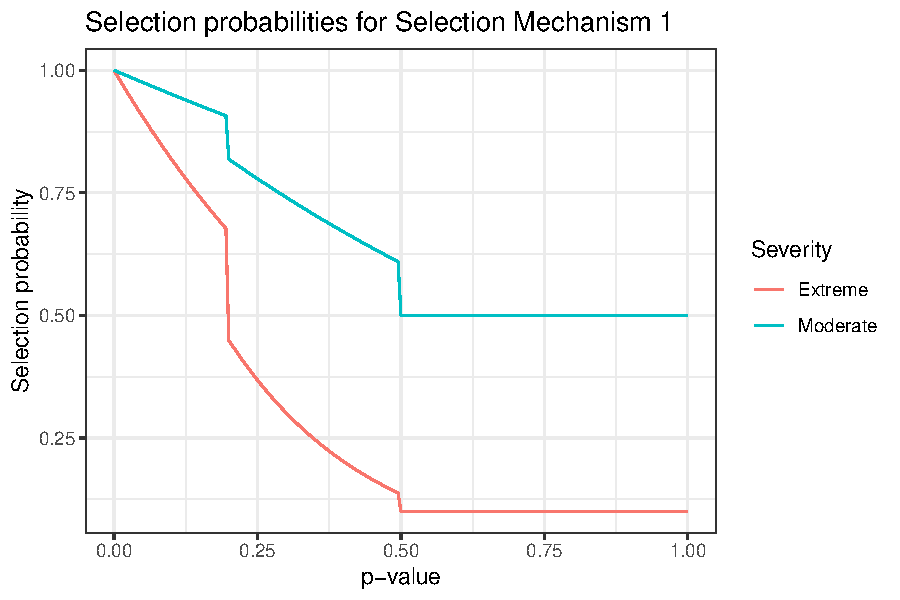
\includegraphics[height = 4in, width = 6in]{SM1.pdf}
\caption{Selection mechanism 1: declining selection probabilities with increasing one-sided p-values. There are steps at $p = .2$ and $p=.5$ and exponential decay between cut-points. 
Selection probability is constant after $p=0.5$.}
\label{fig:SM1}
\end{figure}

\begin{figure}
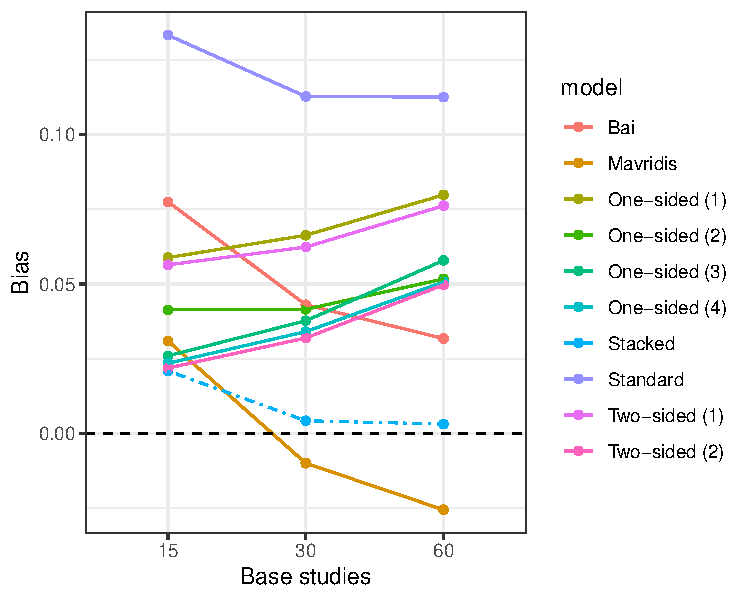
\includegraphics[height = 4in, width = 5in]{extreme_big_bias.pdf}
\caption{Plot of average bias from 200 simulation replications with from Selection mechanism 1 with extreme selection and $\theta = 0.5$.}
\label{fig:func1_extreme_big_bias}
\end{figure}

\begin{figure}
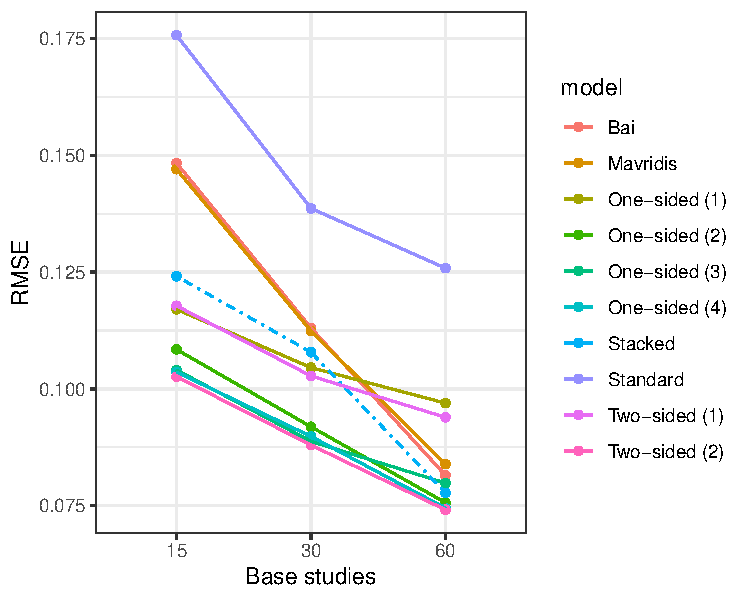
\includegraphics[height = 4in, width = 5in]{extreme_big_rmse.pdf}
\caption{Plot of root(MSE) from 200 simulation replications with from Selection mechanism 1 with extreme selection and $\theta = 0.5$.}
\label{fig:func1_extreme_big_rmse}
\end{figure}

\begin{figure}
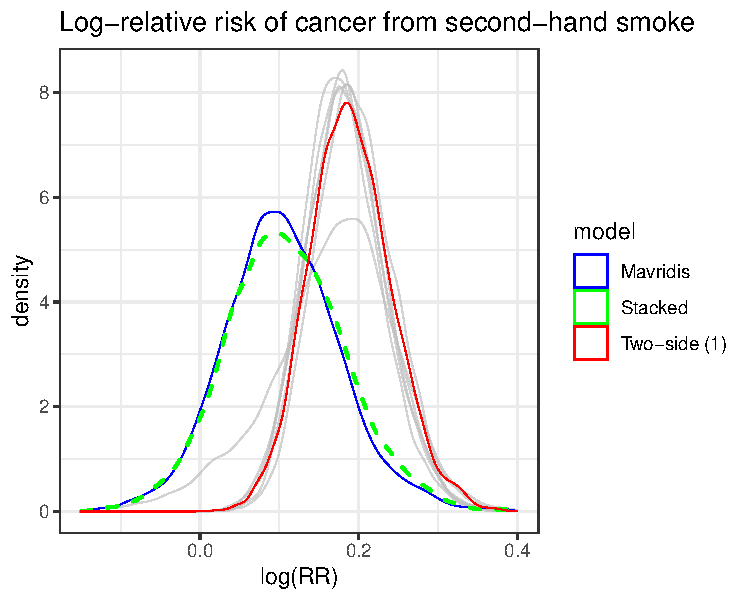
\includegraphics[height = 4in, width = 5in]{hackshaw_post.pdf}
\caption{Posterior distributions of $\theta$ for each selection model using lung cancer data from \citet{hackshaw1997}. Colored lines show models where stacking weight was at least 0.01 (1\%).
Dashed line shows stacked posterior distribution.}
\label{fig:hackshaw}
\end{figure}


\begin{figure}
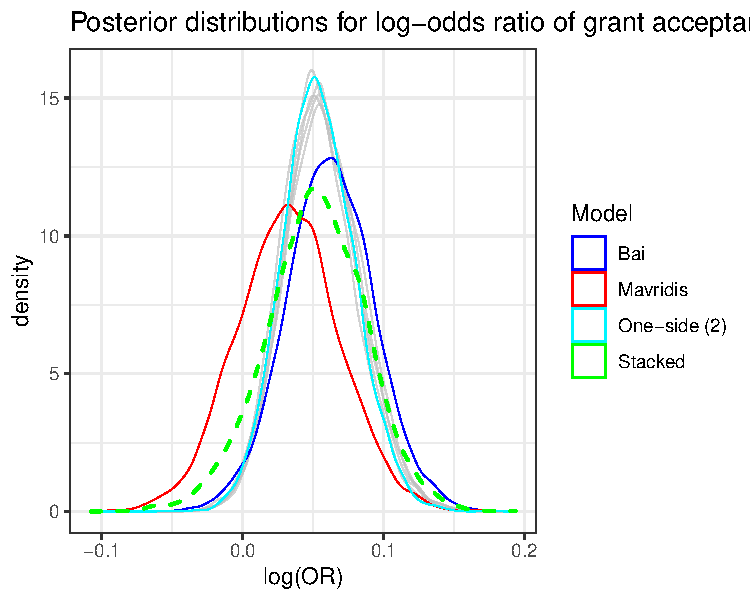
\includegraphics[height = 4in, width = 5in]{bornmann_post.pdf}
\caption{Posterior distributions of $\theta$ for each selection model using grant application data from \citet{bornmann2007gender}. Colored lines show models where stacking weight was at least 0.01 (1\%).
Dashed line is stacked posterior distribution of $\theta$.}
\label{fig:bornmann}
\end{figure}


\begin{figure}
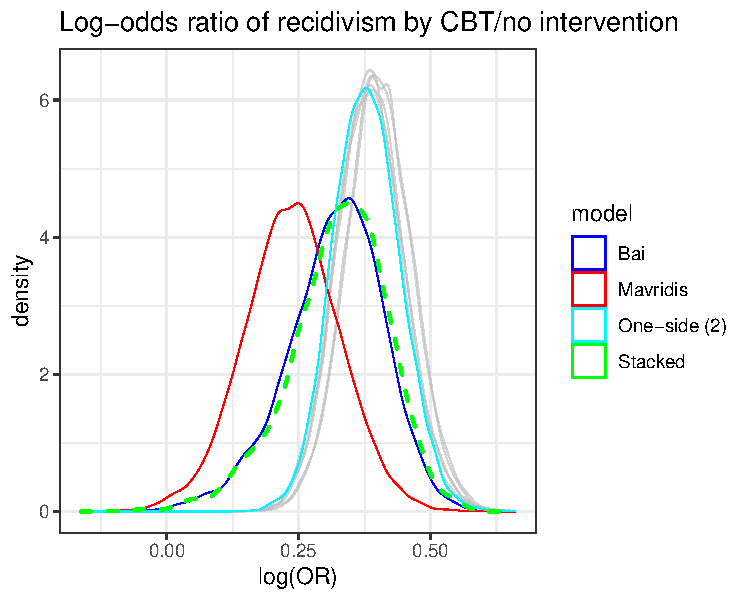
\includegraphics[height = 4in, width = 5in]{landenberger_post.pdf}
\caption{Posterior distributions of $\theta$ for each selection model using recidivism data from \citet{landenberger2005recidivism}. Colored lines show models where stacking weight was at least 0.01 (1\%).
Dashed line shows stacked posterior distribution.}
\label{fig:landenberger}
\end{figure}

%%%% Bibliography
\bibliographystyle{biom}
\bibliography{publication.bias}

\end{document}  



